\documentclass[12pt]{beamer}
\usepackage{Estilos/BeamerFC}
\usepackage{Estilos/ColoresLatex}
\usetheme{Warsaw}
\usecolortheme{seahorse}
%\useoutertheme{default}
\setbeamercovered{invisible}
% or whatever (possibly just delete it)
\setbeamertemplate{section in toc}[sections numbered]
\setbeamertemplate{subsection in toc}[subsections numbered]
\setbeamertemplate{subsection in toc}{\leavevmode\leftskip=3.2em\rlap{\hskip-2em\inserttocsectionnumber.\inserttocsubsectionnumber}\inserttocsubsection\par}
\setbeamercolor{section in toc}{fg=blue}
\setbeamercolor{subsection in toc}{fg=blue}
\setbeamercolor{frametitle}{fg=blue}
\setbeamertemplate{caption}[numbered]

\setbeamertemplate{footline}
\beamertemplatenavigationsymbolsempty
\setbeamertemplate{headline}{}


\makeatletter
\setbeamercolor{section in foot}{bg=gray!30, fg=black!90!orange}
\setbeamercolor{subsection in foot}{bg=blue!30}
\setbeamercolor{date in foot}{bg=black}
\setbeamertemplate{footline}
{
  \leavevmode%
  \hbox{%
  \begin{beamercolorbox}[wd=.333333\paperwidth,ht=2.25ex,dp=1ex,center]{section in foot}%
    \usebeamerfont{section in foot} \insertsection
  \end{beamercolorbox}%
  \begin{beamercolorbox}[wd=.333333\paperwidth,ht=2.25ex,dp=1ex,center]{subsection in foot}%
    \usebeamerfont{subsection in foot}  \insertsubsection
  \end{beamercolorbox}%
  \begin{beamercolorbox}[wd=.333333\paperwidth,ht=2.25ex,dp=1ex,right]{date in head/foot}%
    \usebeamerfont{date in head/foot} {T1 - Segunda presentación} \hspace*{2em}
    \insertframenumber{} / \inserttotalframenumber \hspace*{2ex} 
  \end{beamercolorbox}}%
  \vskip0pt%
}
\makeatother

\makeatletter
\patchcmd{\beamer@sectionintoc}{\vskip1.5em}{\vskip0.8em}{}{}
\makeatother
\usepackage{pifont}
\newcommand{\cmark}{\ding{51}}%
\newcommand{\xmark}{\ding{55}}%

\makeatletter
\setbeamertemplate{footline}
{
  \leavevmode%
  \hbox{%
  \begin{beamercolorbox}[wd=.333333\paperwidth,ht=2.25ex,dp=1ex,center]{section in foot}%
    \usebeamerfont{section in foot} \insertsection
  \end{beamercolorbox}%
  \begin{beamercolorbox}[wd=.333333\paperwidth,ht=2.25ex,dp=1ex,center]{subsection in foot}%
    \usebeamerfont{subsection in foot}  \insertsubsection
  \end{beamercolorbox}%
  \begin{beamercolorbox}[wd=.333333\paperwidth,ht=2.25ex,dp=1ex,right]{date in head/foot}%
    \usebeamerfont{date in head/foot} \insertshortdate{} \hspace*{2em}
    \insertframenumber{} / \inserttotalframenumber \hspace*{2ex} 
  \end{beamercolorbox}}%
  \vskip0pt%
}
\makeatother

\sisetup{
  per-mode=fraction,
  fraction-function=\tfrac
}

\setbeamertemplate{navigation symbols}{}
\date{13 de abril}

% \sisetup{math-rm=\symup,detect-all}
\sisetup{detect-all, math-rm = \ensuremath}

\title{Sesión 7. Física}
\subtitle{Asesoría}

\begin{document}

\maketitle
\fontsize{14}{14}\selectfont
\spanishdecimal{.}

\section*{Contenido}
\frame[allowframebreaks]{\tableofcontents[currentsection, hideallsubsections]}


\section{Sistemas de vectores}
\frame{\tableofcontents[currentsection, hideothersubsections]}



\subsection{Ejercicio 4 Guía}

\begin{frame}
\frametitle{Sistema de vectores del Ejercicio 4}
\begin{figure}
  \centering
  \begin{tikzpicture}[scale=0.5]
  \draw (-4, 0) -- (5, 0);
  \draw (0, -9) -- (0, 5);
  \draw [-stealth, thick, color=carmine] (0, 0) -- (4.17, 4.17) node [above, pos=1] {\small{$F_{1} = \SI{59}{\newton}$}};
  \draw [color=carmine] (0.5, 0) arc(0:45:0.5);
  \node at (2.5, 0.3) [color=carmine] {\small{$\theta_{1} = \ang{45}$}};

  \draw [-stealth, thick, color=electricindigo] (0, 0) -- (1.97, -1.18) node [above, xshift=0.8cm, yshift=-0.7cm] {\small{$F_{2} = \SI{23}{\newton}$}};
  \draw [color=electricindigo] (0.5, 0) arc(360:329:0.5);
  \node at (2.8, -0.5) [color=electricindigo] {\small{$\theta_{2} = \ang{31}$}};
  
  \draw [-stealth, thick, color=officegreen] (0, 0) -- (-0.919, -8.75) node [left, midway] {\small{$F_{3} = \SI{88}{\newton}$}};
  \draw [color=officegreen] (-0.5, 0) arc(180:264:0.5);
  \node at (-2, -0.5) [color=officegreen] {\small{$\theta_{3} = \ang{84}$}};

  \draw [-stealth, thick, color=persimmon] (0, 0) -- (-0.745, 1.52) node [above, xshift=-1cm, yshift=-0.2cm] {\small{$F_{4} = \SI{17}{\newton}$}};
  \draw [thick, color=persimmon] (-0.5, 0) arc(180:116:0.5);
  \node at (-2, 0.5) [color=persimmon] {\small{$\theta_{4} = \ang{64}$}};
\end{tikzpicture}
\end{figure}
\end{frame}
\begin{frame}
\frametitle{Enlistando los vectores}
Recordemos que es conveniente presentar en una tabla los vectores involucrados en el sistema, así como sus magnitudes y ángulos que nos indica el enunciado.
\end{frame}
\begin{frame}
\frametitle{Lista de vectores}
\begin{table}
\centering
\begin{tabular}{c | c | c }
Vector & Magnitud & Ángulo \\ \hline
$\va{F}_{1}$ & $\SI{59}{\newton}$ & $\theta_{1} = \ang{45}$ \\ \hline
$\va{F}_{2}$ & $\SI{23}{\newton}$ & $\theta_{2} = \ang{31}$ \\ \hline
$\va{F}_{3}$ & $\SI{88}{\newton}$ & $\theta_{3} = \ang{84}$ \\ \hline
$\va{F}_{4}$ & $\SI{17}{\newton}$ & $\theta_{4} = \ang{64}$ \\ \hline
\end{tabular}
\end{table}
\end{frame}
\begin{frame}
\frametitle{Cálculo de las componentes}
Procedemos al cálculo de las componentes ocupando el valor del ángulo que se nos indica, revisando con cuidado el signo de la componente a partir del cuadrante en el que se encuentra el vector.
\end{frame}
\begin{frame}
\frametitle{Tabla con las componentes}
\begin{table}
\centering
\begin{tabular}{c | l | l | c}
Componente & Expresión & Sustitución & Valor \\ \hline
$F_{1x}$ & $\cos \theta_{1} \cdot F_{1}$ & $\cos \ang{45} \cdot \SI{59}{\newton}$ & $\SI{41.71}{\newton}$ \\ \hline
$F_{1y}$ & $\sin \theta_{1} \cdot F_{1}$ & $\sin \ang{45} \cdot \SI{59}{\newton}$ & $\SI{41.71}{\newton}$ \\ \hline
$F_{2x}$ & $\cos \theta_{2} \cdot F_{2}$ & $\cos \ang{31} \cdot \SI{23}{\newton}$ & $\SI{19.71}{\newton}$ \\ \hline
$F_{2y}$ & $-\sin \theta_{2} \cdot F_{2}$ & $-\sin \ang{31} \cdot \SI{23}{\newton}$ & $-\SI{11.84}{\newton}$ \\ \hline
\end{tabular}
\end{table}
\end{frame}
\begin{frame}
\frametitle{Tabla con las componentes}
\begin{table}
\centering
\begin{tabular}{c | l | l | c}
Componente & Expresión & Sustitución & Valor \\ \hline
$F_{3x}$ & $-\cos \theta_{3} \cdot F_{3}$ & $-\cos \ang{84} \cdot \SI{88}{\newton}$ & $-\SI{9.19}{\newton}$ \\ \hline
$F_{3y}$ & $-\sin \theta_{3} \cdot F_{3}$ & $-\sin \ang{84} \cdot \SI{88}{\newton}$ & $-\SI{87.51}{\newton}$ \\ \hline
$F_{4x}$ & $-\cos \theta_{4} \cdot F_{4}$ & $-\cos \ang{64} \cdot \SI{17}{\newton}$ & $-\SI{7.45}{\newton}$ \\ \hline
$F_{4y}$ & $\sin \theta_{4} \cdot F_{4}$ & $\sin \ang{64} \cdot \SI{17}{\newton}$ & $\SI{15.27}{\newton}$ \\ \hline
\end{tabular}
\end{table}
\end{frame}
\begin{frame}
\frametitle{Sumando las componentes}
Obtenemos las componentes del vector resultante $F_{R}$ al sumar las componentes tanto en $x$ como en $y$.
\end{frame}
\begin{frame}
\frametitle{Componente en $x$}
Sabemos que:
\pause
\begin{eqnarray*}
\begin{aligned}
F_{Rx} &= \nsum_{i=1}^{4} F_{ix} = \\[0.5em] \pause
&= F_{1x} + F_{2x} + F_{3x} + F_{4x} = \\[0.5em] \pause
&= \SI{41.71}{\newton} {+} \SI{19.71}{\newton} {+} (-\SI{9.19}{\newton}) {+} (-\SI{7.45}{\newton}) = \\[0.5em] \pause
&= \SI{44.78}{\newton}
\end{aligned}
\end{eqnarray*}
\end{frame}
\begin{frame}
\frametitle{Componente en $y$}
Sabemos que:
\pause
\begin{eqnarray*}
\begin{aligned}
F_{Ry} &= \nsum_{i=1}^{4} F_{iy} = \\[0.5em] \pause
&= F_{1y} + F_{2y} + F_{3y} + F_{4y} = \\[0.5em] \pause
&= \SI{41.71}{\newton} {+} (-\SI{11.84}{\newton}) {+} (-\SI{87.51}{\newton}) {+} \SI{15.27}{\newton} = \\[0.5em] \pause
&= -\SI{42.37}{\newton}
\end{aligned}
\end{eqnarray*}
\end{frame}
\begin{frame}
\frametitle{Calculando la magnitud del vector resultante}
Una vez conocidas las componentes $F_{Rx}$ y $F_{Ry}$, podemos obtener la magnitud del vector resultante:
\pause
\begin{eqnarray*}
\begin{aligned}
\abs{F_{R}} &= \sqrt{(F_{Rx})^{2} + (F_{Ry})^{2}} = \\[0.5em] \pause
&= \sqrt{ (\SI{44.78}{\newton})^{2} {+} (-\SI{42.37}{\newton})^{2}} = \\[0.5em] \pause
&= \sqrt{ \SI{2005.24}{\square\newton} + \SI{1795.21}{\square\newton}} = \\[0.5em] \pause
&= \sqrt{\SI{3800.41}{\square\newton}} = \\[0.5em] \pause
&= \SI{61.64}{\newton}
\end{aligned}
\end{eqnarray*}
\end{frame}
\begin{frame}
\frametitle{El ángulo del vector resultante}
Revisando que las componentes $F_{Rx} > 0$ y $F_{Ry} < 0$, por lo que el vector resultante está en el cuadrante IV, \pause con esos valores podemos calcular el valor del ángulo auxiliar $\alpha$ del vector resultante:
\pause
\begin{eqnarray*}
\begin{aligned}
\tan \alpha &= - \dfrac{F_{Ry}}{F_{Rx}} = \pause
  - \dfrac{\SI{42.37}{\newton}}{\SI{44.78}{\newton}} = \pause - 0.9461 \\[0.5em] \pause
\arctan(\tan \alpha) &= \arctan(- 0.94.61) \\[0.5em] \pause
\alpha &= - \ang{43.41}
\end{aligned}
\end{eqnarray*}
\end{frame}
\begin{frame}
\frametitle{El ángulo del vector resultante}
El enunciado nos pide obtener el ángulo del vector resultante $\theta_{R}$ medido desde el eje $x$ positivo, \pause por lo que:
\pause
\begin{eqnarray*}
\begin{aligned}
\theta_{R} &= \ang{360} - \alpha = \\[0.5em] \pause
\theta_{R} &= \ang{360} - \ang{43.41} = \\[0.5em] \pause
\theta_{R} &= \ang{316.59}
\end{aligned}
\end{eqnarray*}
\end{frame}
\begin{frame}[plain]
  \begin{figure}
\centering
\begin{tikzpicture}[scale=0.5]
\draw (-4, 0) -- (5, 0);
\draw (0, -9) -- (0, 5);
\draw [-stealth, thick, color=carmine] (0, 0) -- (4.17, 4.17) node [above, pos=1] {\small{$F_{1}$}};
% \draw [color=carmine] (0.5, 0) arc(0:45:0.5);
% \node at (1.5, 0.4) [color=carmine] {\small{$\theta_{1}$}};

\draw [-stealth, thick, color=electricindigo] (0, 0) -- (1.97, -1.18) node [above, xshift=0.2cm, yshift=-0.2cm] {\small{$F_{2}$}};
% \draw [color=electricindigo] (0.5, 0) arc(360:329:0.5);
% \node at (2, -0.5) [color=electricindigo] {\small{$\theta_{2}$}};

\draw [-stealth, thick, color=officegreen] (0, 0) -- (-0.919, -8.75) node [left, midway] {\small{$F_{2}$}};
% \draw [color=officegreen] (-0.5, 0) arc(180:264:0.5);
% \node at (-2, -0.5) [color=officegreen] {\small{$\theta_{3}$}};

\draw [-stealth, thick, color=persimmon] (0, 0) -- (-0.745, 1.52) node [above, xshift=-0.1cm, yshift=-0.1cm] {\small{$T_{4}$}};
% \draw [thick, color=persimmon] (-0.5, 0) arc(180:116:0.5);
% \node at (-2, 0.5) [color=persimmon] {\small{$\theta_{4}$}};

\draw [thick, color=red] (0.8, 0) arc(360:316.59:0.8);
\node at (2, 0.5) [color=red] {\small$\alpha$};
\draw [-stealth, thick, color=red] (1.6, 0.5) --  (0.8, -0.3);

\draw [-stealth, thick, color=black] (0, 0) -- (4.47, -4.23) node [left, pos=1] {\small{$T_{R}$}};
\draw [thick, color=black] (0.8, 0) arc(0:316.59:0.8);
\node at (0.7, -1.4) [color=black] {\small{$\theta_{R}$}};
\end{tikzpicture}
\end{figure}
\end{frame}

\subsection{Ejercicio 5 Guía}

\begin{frame}
\frametitle{Sistema de vectores del Ejercicio 5}
\begin{figure}
  \centering
  \begin{tikzpicture}[scale=0.5]
  \draw (-10, 0) -- (5, 0);
  \draw (0, -7) -- (0, 7);
  \draw [-stealth, thick, color=red] (0, 0) -- (3.87, 2.32 ) node [above, pos=1] {\small{$\vb{v}_{1} = \SI{59}{\meter\per\second}$}};
  \draw [color=red] (0.5, 0) arc(0:39:0.5);
  \node at (2.5, 0.3) [color=red] {\small{$\theta_{1} = \ang{39}$}};

  \draw [-stealth, thick, color=regalia] (0, 0) -- (2.16, -6.65) node [above, near end, rotate=-72] {\small{$\vb{v}_{2} = \SI{70}{\meter\per\second}$}};
  \draw [color=regalia] (0.5, 0) arc(360:288:0.5);
  \node at (2.5, -0.8) [color=regalia] {\small{$\theta_{2} = \ang{72}$}};
  
  \draw [-stealth, thick, color=rosewood] (0, 0) -- (-9.45, -3.25) node [below, near end, rotate=19] {\small{$\vb{v}_{3} = \SI{100}{\meter\per\second}$}};
  \draw [color=rosewood] (-0.5, 0) arc(180:199:0.5);
  \node at (-3.5, -0.5) [color=rosewood] {\small{$\theta_{3} = \ang{19}$}};

  \draw [-stealth, thick, color=ultramarine] (0, 0) -- (-5.2, 0) node [above, near end] {\small{$\vb{v}_{4} = \SI{52}{\meter\per\second}$}};

  \draw [-stealth, thick, color=persimmon] (0, 0) -- (-1.04, 6.61) node [near end, xshift=-0.2cm, yshift=-0.5cm, rotate=-81] {\small{$\vb{v}_{5} = \SI{67}{\meter\per\second}$}};
  \draw [thick, color=persimmon] (-0.5, 0) arc(180:99:0.5);
  \node at (-2.3, 4) [rotate=-81, color=persimmon] {\small{$\theta_{5} = \ang{81}$}};
  \draw [-stealth, color=persimmon] (-2, 2.6) -- (-0.6, 0.5);
\end{tikzpicture}
\end{figure}
\end{frame}
% \begin{frame}
% \frametitle{Enlistando los vectores}
% Nuevamente presentamos en una tabla los vectores involucrados en el sistema, así como sus magnitudes y ángulos que nos indica el enunciado.
% \end{frame}
% \begin{frame}
% \frametitle{Lista de vectores}
% \begin{table}
% \centering
% \begin{tabular}{c | c | c }
% Vector & Magnitud & Ángulo \\ \hline
% $\vb{v}_{1}$ & $\SI{37}{\meter\per\second}$ & $\theta_{1} = \ang{39}$ \\ \hline
% $\vb{v}_{2}$ & $\SI{70}{\meter\per\second}$ & $\theta_{2} = \ang{72}$ \\ \hline
% $\vb{v}_{3}$ & $\SI{100}{\meter\per\second}$ & $\theta_{3} = \ang{19}$ \\ \hline
% $\vb{v}_{4}$ & $\SI{52}{\meter\per\second}$ & $\theta_{4} = \ang{180}$ \\ \hline
% $\vb{v}_{5}$ & $\SI{67}{\meter\per\second}$ & $\theta_{5} = \ang{81}$ \\ \hline
% \end{tabular}
% \end{table}
% \end{frame}
% \begin{frame}
% \frametitle{Cálculo de las componentes}
% Calculamos las componentes ocupando el valor del ángulo que se nos indica, revisando con cuidado el signo de la componente a partir del cuadrante en el que se encuentra el vector.
% \end{frame}
% \begin{frame}
% \frametitle{Tabla con las componentes}
% \begin{table}
% \centering
% \begin{tabular}{c | l | l | c}
% Componente & Expresión & Sustitución & Valor \\ \hline
% $v_{1x}$ & $\cos \theta_{1} \cdot v_{1}$ & $\cos \ang{39} \cdot \SI{37}{\meter\per\second}$ & $\SI{28.75}{\meter\per\second}$ \\ \hline
% $v_{1y}$ & $\sin \theta_{1} \cdot v_{1}$ & $\sin \ang{39} \cdot \SI{37}{\meter\per\second}$ & $\SI{23.28}{\meter\per\second}$ \\ \hline
% $v_{2x}$ & $\cos \theta_{2} \cdot v_{2}$ & $\cos \ang{72} \cdot \SI{70}{\meter\per\second}$ & $\SI{21.63}{\meter\per\second}$ \\ \hline
% $v_{2y}$ & $-\sin \theta_{2} \cdot v_{2}$ & $-\sin \ang{72} \cdot \SI{70}{\meter\per\second}$ & $-\SI{66.57}{\meter\per\second}$ \\ \hline
% \end{tabular}
% \end{table}
% \end{frame}
% \begin{frame}
% \frametitle{Tabla con las componentes}
% \begin{table}
% \centering
% \begin{tabular}{c | l | l | c}
% Componente & Expresión & Sustitución & Valor \\ \hline
% $v_{3x}$ & $-\cos \theta_{3} \cdot v_{3}$ & $-\cos \ang{19} \cdot \SI{100}{\meter\per\second}$ & $-\SI{94.55}{\meter\per\second}$ \\ \hline
% $v_{3y}$ & $-\sin \theta_{3} \cdot v_{3}$ & $-\sin \ang{19} \cdot \SI{100}{\meter\per\second}$ & $-\SI{32.55}{\meter\per\second}$ \\ \hline
% $v_{4x}$ & $-\cos \theta_{4} \cdot v_{4}$ & $-\cos \ang{180} \cdot \SI{52}{\meter\per\second}$ & $-\SI{52}{\meter\per\second}$ \\ \hline
% $v_{4y}$ & $\sin \theta_{4} \cdot v_{4}$ & $\sin \ang{180} \cdot \SI{52}{\meter\per\second}$ & $\SI{0}{\meter\per\second}$ \\ \hline
% \end{tabular}
% \end{table}
% \end{frame}
% \begin{frame}
% \frametitle{Tabla con las componentes}
% \begin{table}
% \centering
% \begin{tabular}{c | l | l | c}
% Componente & Expresión & Sustitución & Valor \\ \hline
% $v_{5x}$ & $-\cos \theta_{5} \cdot v_{5}$ & $-\cos \ang{81} \cdot \SI{67}{\meter\per\second}$ & $-\SI{10.48}{\meter\per\second}$ \\ \hline
% $v_{5y}$ & $\sin \theta_{5} \cdot v_{5}$ & $\sin \ang{81} \cdot \SI{67}{\meter\per\second}$ & $\SI{66.17}{\meter\per\second}$ \\ \hline
% \end{tabular}
% \end{table}
% \end{frame}
% \begin{frame}
% \frametitle{Sumando las componentes}
% Obtenemos las componentes del vector resultante $v_{R}$ al sumar las componentes tanto en $x$ como en $y$.
% \end{frame}
% \begin{frame}
% \frametitle{Componente en $x$}
% Sabemos que:
% \pause
% \begin{eqnarray*}
% \begin{aligned}
% &v_{Rx} = \nsum_{i=1}^{5} v_{ix} = \pause
% v_{1x} + v_{2x} + v_{3x} + v_{4x} + v_{5x} = \\[0.5em] \pause
% &= \SI{28.75}{\meter\per\second} {+} \SI{21.63}{\meter\per\second} {+} (-\SI{94.55}{\meter\per\second}) + \\[0.5em] 
% &+ (-\SI{52}{\meter\per\second}) {+} (-\SI{10.48}{\meter\per\second}) = \\[0.5em] \pause
% &= -\SI{106.65}{\meter\per\second}
% \end{aligned}
% \end{eqnarray*}
% \end{frame}
% \begin{frame}
% \frametitle{Componente en $y$}
% Sabemos que:
% \pause
% \begin{eqnarray*}
% \begin{aligned}
% &v_{Ry} = \nsum_{i=1}^{5} v_{iy} = \pause
% v_{1y} + v_{2y} + v_{3y} + v_{4y} + v_{5y} = \\[0.5em] \pause
% &= \SI{23.28}{\meter\per\second} {+} (-\SI{66.57}{\meter\per\second}) {+} (-\SI{32.55}{\meter\per\second}) + \\[0.5em] 
% &+ \SI{0}{\meter\per\second} {+} \SI{66.17}{\meter\per\second} = \\[0.5em] \pause
% &= -\SI{9.67}{\meter\per\second}
% \end{aligned}
% \end{eqnarray*}
% \end{frame}
% \begin{frame}
% \frametitle{Calculando la magnitud del vector resultante}
% Una vez conocidas las componentes $v_{Rx}$ y $v_{Ry}$, podemos obtener la magnitud del vector resultante:
% \pause
% \begin{eqnarray*}
% \begin{aligned}
% \abs{v_{R}} &= \sqrt{(v_{Rx})^{2} + (v_{Ry})^{2}} = \\[0.5em] \pause
% &= \sqrt{ (-\SI{106.65}{\meter\per\second})^{2} {+} (-\SI{9.67}{\meter\per\second})^{2}} = \\[0.5em] \pause
% &= \sqrt{ \SI{11374.22}{\square\meter\per\square\second} + \SI{93.50}{\square\meter\per\square\second}} = \\[0.5em] \pause
% &= \sqrt{\SI{11467.72}{\square\meter\per\square\second}} = \\[0.5em] \pause
% &= \SI{107.08}{\meter\per\second}
% \end{aligned}
% \end{eqnarray*}
% \end{frame}
% \begin{frame}
% \frametitle{El ángulo del vector resultante}
% Revisando que las componentes $v_{vRx} < 0$ y $v_{Ry} < 0$, por lo que el vector resultante está en el cuadrante III, \pause con esos valores podemos calcular el valor del ángulo auxiliar $\alpha$ del vector resultante:
% \pause
% \begin{eqnarray*}
% \begin{aligned}
% \tan \alpha &= - \dfrac{v_{Ry}}{v_{Rx}} = \pause
%   - \dfrac{\SI{9.67}{\meter\per\second}}{\SI{106.65}{\meter\per\second}} = \pause - 0.0906 \\[0.5em] \pause
% \arctan(\tan \alpha) &= \arctan(- 0.0906) \\[0.5em] \pause
% \alpha &= - \ang{5.18}
% \end{aligned}
% \end{eqnarray*}
% \end{frame}
% \begin{frame}
% \frametitle{El ángulo del vector resultante}
% El enunciado nos pide obtener el ángulo del vector resultante $\theta_{R}$ medido desde el eje $x$ positivo, \pause por lo que:
% \pause
% \begin{eqnarray*}
% \begin{aligned}
% \theta_{R} &= \ang{270} - \alpha = \\[0.5em] \pause
% \theta_{R} &= \ang{270} - \ang{5.18} = \\[0.5em] \pause
% \theta_{R} &= \ang{264.82}
% \end{aligned}
% \end{eqnarray*}
% \end{frame}
% \begin{frame}[plain]
%   \begin{figure}
% \centering
% \begin{tikzpicture}[scale=0.5]
% \draw (-11, 0) -- (5, 0);
% \draw (0, -10) -- (0, 7);
% \draw [-stealth, thick, color=red] (0, 0) -- (3.87, 2.32 ) node [above, pos=1] {\small{$\vb{v}_{1}$}};
% % \draw [color=red] (0.5, 0) arc(0:39:0.5);
% % \node at (2.5, 0.3) [color=red] {\small{$\theta_{1} = \ang{39}$}};

% \draw [-stealth, thick, color=regalia] (0, 0) -- (2.16, -6.65) node [above, near end, rotate=-72] {\small{$\vb{v}_{2}$}};
% % \draw [color=regalia] (0.5, 0) arc(360:288:0.5);
% % \node at (2.5, -0.8) [color=regalia] {\small{$\theta_{2} = \ang{72}$}};

% \draw [-stealth, thick, color=rosewood] (0, 0) -- (-9.45, -3.25) node [below, near end, rotate=19] {\small{$\vb{v}_{3}$}};
% % \draw [color=rosewood] (-0.5, 0) arc(180:199:0.5);
% % \node at (-3.5, -0.5) [color=rosewood] {\small{$\theta_{3} = \ang{19}$}};

% \draw [-stealth, thick, color=ultramarine] (0, 0) -- (-5.2, 0) node [above, near end] {\small{$\vb{v}_{4}$}};

% \draw [-stealth, thick, color=persimmon] (0, 0) -- (-1.04, 6.61) node [near end, xshift=-0.2cm, yshift=-0.5cm, rotate=-81] {\small{$\vb{v}_{5}$}};
% % \draw [thick, color=persimmon] (-0.5, 0) arc(180:99:0.5);
% % \node at (-2.3, 4) [rotate=-81, color=persimmon] {\small{$\theta_{5} = \ang{81}$}};
% % \draw [-stealth, color=persimmon] (-2, 2.6) -- (-0.6, 0.5);

% \draw [-stealth, thick, color=black] (0, 0) -- (-0.966, -10.64) node [left, near end] {$\vb{v}_{R}$};
% \draw [thick, color=black] (0.5, 0) arc(0:264:0.5);
% \node at (-1, -1.5) [color=black] {\small{$\theta_{R}$}};
% \draw [thick, color=ao] (0, -4.5) arc(270:264:4.5);
% \node at (0.5, -4.8) [color=ao] {\small{$\alpha$}};
% \end{tikzpicture}
% \end{figure}
% \end{frame}

\section{Primera condición de equilibrio}
\frame{\tableofcontents[currentsection, hideothersubsections]}
\subsection{Diagrama de cuerpo libre}

\begin{frame}
\frametitle{¿Qué es el diagrama de cuerpo libre?}
Un \textocolor{carmine}{diagrama de cuerpo libre (DCL)} es una herramienta utilizada en física para visualizar las fuerzas que actúan sobre un objeto en un sistema.
\end{frame}
\begin{frame}
\frametitle{¿Qué es el diagrama de cuerpo libre?}
Se utiliza para aislar el objeto de su entorno y mostrar todas las fuerzas externas que actúan sobre él, así como la dirección y magnitud de cada fuerza.
\end{frame}
\begin{frame}
\frametitle{¿Qué es el diagrama de cuerpo libre?}
Un \textocolor{carmine}{DCL} típicamente consiste en un dibujo del objeto aislado de su entorno, con todas las fuerzas externas que actúan sobre él representadas por vectores, es decir, flechas que indican la dirección y magnitud de cada fuerza.
\end{frame}
\begin{frame}
\frametitle{¿Qué es el diagrama de cuerpo libre?}
Estas fuerzas pueden incluir la gravedad, la fricción, la tensión, la fuerza normal y cualquier otra fuerza externa que pueda afectar el movimiento del objeto.
\end{frame}
\begin{frame}
\frametitle{¿Para qué sirve un diagrama de cuerpo libre?}
El objetivo de un \textocolor{carmine}{DCL} es analizar el movimiento de un objeto y determinar las fuerzas que actúan sobre él.
\end{frame}
\begin{frame}
\frametitle{¿Qué es el diagrama de cuerpo libre?}
Al identificar todas las fuerzas externas que actúan sobre el objeto y representarlas de manera clara y concisa en un \textocolor{carmine}{DCL}, es posible calcular la aceleración del objeto y predecir su movimiento.
\end{frame}
\begin{frame}
\frametitle{¿Qué es el diagrama de cuerpo libre?}
Los \textocolor{carmine}{DCL} son particularmente útiles en situaciones en las que las fuerzas que actúan sobre un objeto son complejas y no son fácilmente visibles a simple vista. 
\end{frame}


\subsection{Ejercicios - Guía}

\begin{frame}
\frametitle{Lo que hay que obtener}
Para cada problema determina:
\pause
\setbeamercolor{item projected}{bg=ao,fg=bananayellow}
\setbeamertemplate{enumerate items}{%
\usebeamercolor[bg]{item projected}%
\raisebox{1.5pt}{\colorbox{bg}{\color{fg}\footnotesize\insertenumlabel}}%
}
\begin{enumerate}[<+->]
\item El diagrama de cuerpo libre.
\item Las tensiones que se indican en cada problema.
\end{enumerate}
\end{frame}

\subsection*{Ejercicio 6}

\begin{frame}
\frametitle{Enunciado del Ejercicio 6}
Dos cuerdas se extienden entre dos postes. Una persona de \SI{65}{\kilo\gram} cuelga de ellas como se muestra en la siguiente figura.
\\
\bigskip
\pause
Encuentra la tensión en cada una de las cuerdas.
\end{frame}
\begin{frame}
\frametitle{Figura del Ejercicio 6}
\begin{figure}
  \centering
  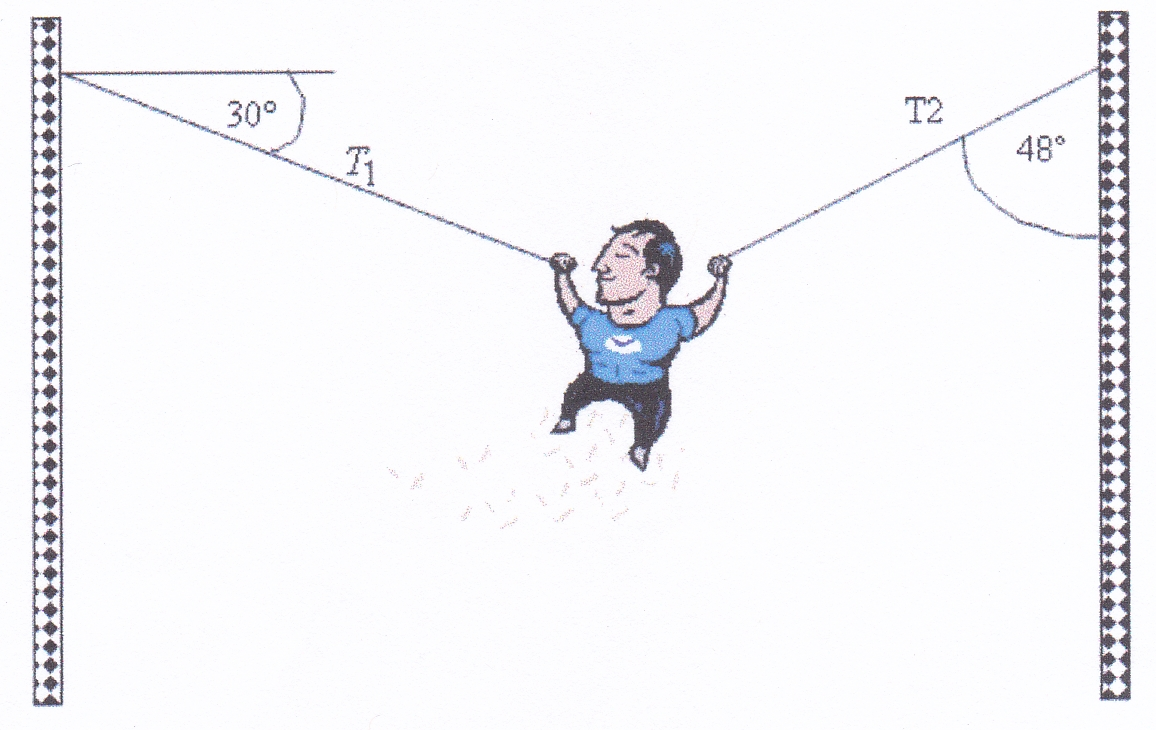
\includegraphics[scale=1]{Imagenes/DCL_Problema_06.png}
\end{figure}
\end{frame}
\begin{frame}
\frametitle{Revisando el enunciado}
Tomemos en cuenta que el ejercicio nos indica que la persona tiene una masa de \SI{65}{\kilo\gram}, por lo que la fuerza debida a la aceleración de la gravedad es:
\pause
\begin{eqnarray*}
\begin{aligned}
F &= - m \, g = \pause - \SI{65}{\kilogram} \cdot \SI{9.81}{\meter\per\square\second} = \\[0.5em] \pause
&= - \SI{637.65}{\newton}
\end{aligned}
\end{eqnarray*}
\pause
Esta fuerza la representamos con un vector cuya dirección está en el eje $y$ negativo.
\end{frame}
\begin{frame}
\frametitle{Diagrama de cuerpo libre}
\begin{figure}
\centering
\begin{tikzpicture}[scale=0.7]
  
  \draw (-5, 0) -- (5, 0);
  \draw [-stealth, thick, color=ao] (0, 0) -- (0, -6.37) node [right, midway] {\small{$-m \, g$}};

  \pause
  \draw (-4.31, 2.94) -- (-3, 2.94);
  \draw [color=red] (-3.81, 2.94) arc (0:-30:0.5);
  \node at (-3, 2.5) [color=red] {\small{$\theta_{1}$}};
  \draw [-stealth, thick, color=red] (0, 0) -- (-4.31, 2.94) node [above, midway] {\small{$T_{1}$}};
  \node at (-5.5, 2.3) {\small{$\theta_{1} = \ang{30}$}};

  \pause
  \draw [color=red] (-0.5, 0) arc(180:150:0.5);
  \node at (-1.5, 0.4) [color=red] {\small{$\theta_{1}$}};

  \pause
  \draw (4.31, 3.88) -- (4.31, 2.5);
  \draw (4.31, 3.4) arc(270:222:0.5);
  \node at (3.9, 3) {\small{$\alpha$}};
  \node at (5.7, 3.3) {\small{$\alpha = \ang{48}$}};
  \draw [-stealth, thick, color=red] (0, 0) -- (4.31, 3.88) node [above, midway] {\small{$T_{2}$}};
  \pause
  \node at (5.7, 2.6) {\small{$\theta_{2} = \ang{42}$}};
  \draw (4.31, 3.88) -- (3, 3.88);
  \draw [color=red] (3.81, 3.88) arc (180:222:0.5);
  \node at (3, 3.35) [color=red] {\small{$\theta_{2}$}};

  \draw [color=red] (0.5, 0) arc(0:42:0.5);
  \node at (1.5, 0.4) [color=red] {\small{$\theta_{2}$}};

  \pause
  \node at (6.3, 1.9) {\small{$\alpha + \theta_{2} = \ang{90}$}};
\end{tikzpicture}
\end{figure}
\end{frame}
\begin{frame}
\frametitle{Condiciones de equilibrio}
Sabemos que si el sistema está en equilibrio, la suma de las componentes de las fuerzas tano en la dirección $x$, como en $y$ valen cero:
\pause
\begin{eqnarray*}
\begin{aligned}
\nsum F_{x} &= 0 \\[0.5em] \pause 
\nsum F_{y} &= 0
\end{aligned}
\end{eqnarray*}
\end{frame}
\begin{frame}
\frametitle{Condiciones de equilibrio}
Tendremos entonces:
\begin{eqnarray*}
\begin{aligned}
\nsum F_{x} &= -\cos \ang{30} \cdot T_{1} + \cos \ang{42} \cdot T_{2} = 0 \\[0.5em] \pause
\nsum F_{x} &= -0.866 \cdot T_{1} + 0.7431 \cdot T_{2} = 0 \\[0.5em] \pause
\nsum F_{y} &= \sen \ang{30} \cdot T_{1} + \sin \ang{42} \cdot T_{2} - m \, g = 0 \\[0.5em] \pause
\nsum F_{y} &= 0.5 \cdot T_{1} + 0.6691 \cdot T_{2} - \SI{637.65}{\newton} = 0 \\[0.5em] \pause
\end{aligned}
\end{eqnarray*}
\end{frame}
\begin{frame}
\frametitle{Sistema de dos ecuaciones}
Con las expresiones anteriores se obtiene un sistema de dos ecuaciones simultáneas con dos incógnitas:
\pause
\begin{align*}
-0.866 \cdot T_{1} + 0.7431 \cdot T_{2} &= 0 \\[0.5em]
0.5 \cdot T_{1} + 0.6691 \cdot T_{2} - \SI{637.65}{\newton} &= 0
\end{align*}
\pause
De donde podemos utilizar cualquier técnica para resolver este sistema simultáneo de dos ecuaciones.
\end{frame}
\begin{frame}
\frametitle{Resolviendo el sistema de ecuaciones}
Acomodando los términos del sistema, se tiene:
\pause
\begin{align}
-0.866 \cdot T_{1} + 0.7431 \cdot T_{2} &= 0 \label{eq:ecuacion_01} \\[0.5em]
0.5 \cdot T_{1} + 0.6691 \cdot T_{2} &= \SI{637.65}{\newton} \label{eq:ecuacion_02}
\end{align}
\pause
De la ecuación (\ref{eq:ecuacion_01}) despejamos el valor de $T_{2}$:
\pause
\begin{eqnarray*}
\begin{aligned}
T_{2} = \dfrac{0.866}{0.7431} \cdot T_{1} = \pause 1.1653 \cdot T_{1}
\end{aligned}
\end{eqnarray*}
\end{frame}
\begin{frame}
\frametitle{Resolviendo las tensiones}
El valor anterior de $T_{2}$ lo sustituimos en la ecuación (\ref{eq:ecuacion_02}), para obtener $T_{1}$:
\pause
\begin{eqnarray*}
\begin{aligned}
0.5 \cdot T_{1} + 0.6691 \cdot (1.1653 \, T_{1}) &= \SI{637.65}{\newton} \\[0.5em] \pause
0.5 \cdot T_{1} + 0.7797 \cdot T_{1} &= \SI{637.65}{\newton} \\[0.5em] \pause
1.2797 \cdot T_{1} &= \SI{637.65}{\newton} \\[0.5em] \pause
T_{1} &= \dfrac{\SI{637.65}{\newton}}{1.2797} = \pause \SI{498.28}{\newton}
\end{aligned}
\label{eq:ecuacion_03}
\end{eqnarray*}
\end{frame}
\begin{frame}
\frametitle{Obteniendo el segundo término}
Una vez obtenido $T_{1}$ usamos este valor para calcular $T_{2}$, para ello ocupamos la ecuación (\ref{eq:ecuacion_01})
\pause
\begin{eqnarray*}
\begin{aligned}
-0.866 \cdot T_{1} + 0.7431 \cdot T_{2} &= 0 \\[0.5em] \pause
-0.866 \cdot \SI{498.28}{\newton} + 0.7431 \cdot T_{2} &= 0
\end{aligned}
\end{eqnarray*}
\end{frame}
\begin{frame}
\frametitle{Obteniendo el segundo término}
Reacomodamos los términos:
\pause
\begin{eqnarray*}
\begin{aligned}
0.7431 \cdot T_{2} &= 0.866 \cdot \SI{498.28}{\newton} \\[0.5em] \pause
T_{2} &= \dfrac{0.866}{0.7431} \cdot \SI{498.28}{\newton} \\[0.5em] \pause
T_{2} &= 1.1653 \cdot \SI{498.28}{\newton} \\[0.5em] \pause
T_{2} &= \SI{580.68}{\newton}
\end{aligned}
\end{eqnarray*}
\end{frame}

\end{document}